\documentclass[spanish,]{book}
\usepackage{lmodern}
\usepackage{amssymb,amsmath}
\usepackage{ifxetex,ifluatex}
\usepackage{fixltx2e} % provides \textsubscript
\ifnum 0\ifxetex 1\fi\ifluatex 1\fi=0 % if pdftex
  \usepackage[T1]{fontenc}
  \usepackage[utf8]{inputenc}
\else % if luatex or xelatex
  \ifxetex
    \usepackage{mathspec}
  \else
    \usepackage{fontspec}
  \fi
  \defaultfontfeatures{Ligatures=TeX,Scale=MatchLowercase}
\fi
% use upquote if available, for straight quotes in verbatim environments
\IfFileExists{upquote.sty}{\usepackage{upquote}}{}
% use microtype if available
\IfFileExists{microtype.sty}{%
\usepackage{microtype}
\UseMicrotypeSet[protrusion]{basicmath} % disable protrusion for tt fonts
}{}
\usepackage{hyperref}
\hypersetup{unicode=true,
            pdftitle={Fundamentos de Investigación II},
            pdfauthor={Luis Eudave},
            pdfborder={0 0 0},
            breaklinks=true}
\urlstyle{same}  % don't use monospace font for urls
\ifnum 0\ifxetex 1\fi\ifluatex 1\fi=0 % if pdftex
  \usepackage[shorthands=off,main=spanish]{babel}
\else
  \usepackage{polyglossia}
  \setmainlanguage[]{spanish}
\fi
\usepackage{natbib}
\bibliographystyle{apalike}
\usepackage{longtable,booktabs}
\usepackage{graphicx,grffile}
\makeatletter
\def\maxwidth{\ifdim\Gin@nat@width>\linewidth\linewidth\else\Gin@nat@width\fi}
\def\maxheight{\ifdim\Gin@nat@height>\textheight\textheight\else\Gin@nat@height\fi}
\makeatother
% Scale images if necessary, so that they will not overflow the page
% margins by default, and it is still possible to overwrite the defaults
% using explicit options in \includegraphics[width, height, ...]{}
\setkeys{Gin}{width=\maxwidth,height=\maxheight,keepaspectratio}
\IfFileExists{parskip.sty}{%
\usepackage{parskip}
}{% else
\setlength{\parindent}{0pt}
\setlength{\parskip}{6pt plus 2pt minus 1pt}
}
\setlength{\emergencystretch}{3em}  % prevent overfull lines
\providecommand{\tightlist}{%
  \setlength{\itemsep}{0pt}\setlength{\parskip}{0pt}}
\setcounter{secnumdepth}{5}
% Redefines (sub)paragraphs to behave more like sections
\ifx\paragraph\undefined\else
\let\oldparagraph\paragraph
\renewcommand{\paragraph}[1]{\oldparagraph{#1}\mbox{}}
\fi
\ifx\subparagraph\undefined\else
\let\oldsubparagraph\subparagraph
\renewcommand{\subparagraph}[1]{\oldsubparagraph{#1}\mbox{}}
\fi

%%% Use protect on footnotes to avoid problems with footnotes in titles
\let\rmarkdownfootnote\footnote%
\def\footnote{\protect\rmarkdownfootnote}

%%% Change title format to be more compact
\usepackage{titling}

% Create subtitle command for use in maketitle
\providecommand{\subtitle}[1]{
  \posttitle{
    \begin{center}\large#1\end{center}
    }
}

\setlength{\droptitle}{-2em}

  \title{Fundamentos de Investigación II}
    \pretitle{\vspace{\droptitle}\centering\huge}
  \posttitle{\par}
    \author{Luis Eudave}
    \preauthor{\centering\large\emph}
  \postauthor{\par}
      \predate{\centering\large\emph}
  \postdate{\par}
    \date{2020-09-23}

\usepackage{booktabs}
\usepackage{longtable}

\begin{document}
\maketitle

{
\setcounter{tocdepth}{1}
\tableofcontents
}
\chapter{Introducción a la probabilidad}\label{probability}

Para muchas personas, cuando piensan en estadística se les viene esto a
la mente: calcular promedios, recopilar datos, elaborar gráficos y
ponerlos todos en un informe en algún lugar. Mas o menos como
coleccionar sellos o cucharillas, pero con números. Sin embargo, las
estadística cubre mucho más que eso. De hecho, la estadística
descriptiva es una de las partes más pequeñas de la estadística, y una
de las menos poderosas (en cuanto a las conclusiones que puede aportar).
La parte más importante y más útil de la estadística es aquella que que
permite hacer \emph{inferencias} sobre los datos.

Una vez contemplada las estadística en estos términos, -que la
estadística está ahí para ayudarnos a hacer inferencias a partir de
datos- podemos ver ejemplos de ella en todas partes. Por ejemplo, aquí
hay un pequeño extracto de un periódico mexicano:

\begin{quote}
``Tengo un trabajo difícil'', dijo el Presidente mexicano en respuesta a
una encuesta que encontró que su gobierno ha pasado de gozar los mayores
índices de popularidad en la historia (\textgreater{}70\%) a un 38 por
ciento.
\end{quote}

Este tipo de comentarios suele pasar como completamente irrelevante en
los periódicos o en la vida cotidiana, pero pensemos brevemento sobre lo
que implica. Una compañía encuestadora ha realizado una encuesta,
presumiblemente una muy grande porque tiene los medios y puede
permitírselo. Imaginemos que llamaron a 1.000 votantes al azar, y 380
(38\%) de ellos afirmaron que tenían la intención de votar por el
Presidente. En las últimas elecciones federals, la Instituto Electoral
Mexicano confirmó la participación de 56.611.027 votantes; por lo tanto,
las opiniones de los 56.610.027 votantes restantes (aproximadamente el
99.998\% de los votantes) siguen siendo desconocidas para la
encuestadora (y para nosotros). Aún suponiendo que nadie mintió en la
encuesta, lo único que podemos decir con un 100\% de seguridad es que el
verdadero voto primario al Presidente está en algún lugar entre
380/56.611.027 (aproximadamente el 0.0007\%) y 56.610.307/56.611.027
(alrededor del 99.9987\%), lo cual no aporta mucho. Entonces, ¿sobre qué
base es legítimo para la empresa encuestadora, el periódico y el
lectores concluir que la intención de voto al Presidente mexicano fue de
sólo el 38\%?

La respuesta a la pregunta es bastante obvia: si llamo a 1.000 personas
al azar, y 380 de ellas dicen tienen la intención de votar por el
Presidente, entonces parece muy poco probable que estas sean las
\emph{únicas} 380 personas del todo el público votante que realmente
tiene la intención de hacerlo. En otras palabras, suponemos que los
datos recopilados por la empresa encuestadora son bastante
representativos de la población en general. ¿Pero qué tan
representativo? ¿Nos sorprendería descubrir que la verdadera intención
de voto es en realidad del 34\%? ¿39\%? ¿57\%? En este punto nuestración
intuición comienza a romperse un poco. Nadie se sorprendería si fuese el
34\%, y todos lo harían con un 57\%, pero es un poco difícil decir si el
39\% es plausible. Necesitamos herramientas más poderosas que solo el
mirar los números y adivinar.

\textbf{\emph{La estadística inferencial}} proporciona las herramientas
que necesitamos para responder a este tipo de preguntas, y ya que este
tipo de preguntas se encuentran en el corazón del quehacer científico,
ocupan una parte sustancial de cada curso introductorio sobre
estadística y métodos de investigación. Sin embargo, la teoría sobre la
estadística inferencial está construida sobre la \textbf{\emph{teoría de
probabilidad}}. Y es a la teoría de la probabilidad a la que ahora
debemos prestar atención. La discusión de la teoría de la probabilidad
en esta asignatura será básicamente de fondo: no hay mucho contenido
estadístico \emph{per se} en este capítulo. Sin embargo, debido a que
gran parte de la estadística se sustenta en la teoría de la
probabilidad, merece la pena ir cubriendo algunos de los conceptos
básicos.

\section{¿Cómo de diferentes son la probabilidad y la
estadística?}\label{probstats}

Antes de comenzar a hablar sobre la teoría de la probabilidad, es útil
pensar un momento en la relación que existe entre probabilidad y
estadística. Las dos disciplinas están estrechamente relacionadas, pero
no son idénticas. La teoría de la probabilidad es ``la doctrina de las
posibilidades''. Es una rama de las matemáticas que te dice con qué
frecuencia sucederán diferentes tipos de eventos. Por ejemplo, todas
estas preguntas son cosas que puedes responder usando la teoría de la
probabilidad:

\begin{itemize}
\tightlist
\item
  ¿Cuáles son las probabilidades de que al lanzar una moneda salga cara
  10 veces seguidas?
\item
  Si lanzo dos dados de seis caras, ¿qué probabilidad hay de que tire
  dos seises?
\item
  ¿Qué probabilidad hay de que cinco cartas extraídas de un mazo
  perfectamente barajado sean todas de corazones?
\item
  ¿Cuál es la probabilidad de que gane la lotería?
\end{itemize}

Hay que tener en cuenta que todas estas preguntas tienen algo en común.
En cada caso, existe y se conoce una ``verdad sobre el mundo'', y la
pregunta se refiere más bien al ``qué tipo de eventos'' sucederán. En la
primera pregunta que \emph{sé} que la moneda es justa (no es más pesada
por uno de los lados, sesgando el resultado), por lo que hay un 50\% de
probabilidad de que cualquier lanzamiento de moneda salga cara. En la
segunda pregunta, \emph{sé} que la probabilidad de sacar un 6 en un solo
dado es de 1 en 6. En la tercera pregunta \emph{sé} que la baraja se
baraja correctamente (no hay un acomodo de cartas). Y en la cuarta
pregunta, \emph{sé} que la lotería sigue unas reglas específicas. El
punto clave aquí es que las preguntas probabilísticas comienzan con un
\textbf{\emph{modelo}} conocido del mundo, y usamos ese modelo para
hacer algunos cálculos. El modelo subyacente puede ser bastante simple.
Por ejemplo, en el ejemplo de lanzar monedas, podemos escribir el modelo
de esta manera: \[
P(\mbox{cara}) = 0.5
\] que puedes leer como ``la probabilidad de que salga cara es 0.5''.
Como veremos más adelante, de la misma manera que los porcentajes son
números que van del 0\% al 100\%, las probabilidades son solo números
que van del 0 al 1. Cuando usamos este modelo de probabilidad para
responder a la primera pregunta, en realidad no sé exactamente qué va a
ocurrir. Tal vez obtenga 10 caras, como dice la pregunta. Pero quizás
salgan sólo tres caras. Esta es la clave: con la teoría de la
probabilidad, se conoce el \emph{modelo}, pero no los \emph{datos}.

Hemos visto lo que es la probabilidad. ¿Qué hay de la estadística? Las
preguntas en estadística funcionan al revés. En estadística, nosotros
\emph{no} sabemos la verdad sobre el mundo. Todo lo que tenemos son los
datos, y es a partir de esos datos que queremos \emph{aprender} sobre la
verdad del mundo. Las preguntas estadísticas tienden a parecerse más a
estas:

\begin{itemize}
\tightlist
\item
  Si mi amigo lanza una moneda 10 veces y obtiene 10 caras, ¿me está
  engañando?
\item
  Si las primeras cinco cartas de la parte superior del mazo son todas
  de corazones, ¿qué tan probable es que se haya barajado el mazo?
\item
  Si el hijo del comisionado de la lotería gana la lotería, ¿qué tan
  probable es que el sorteo esté amañado?
\end{itemize}

Esta vez, lo único que tenemos son datos. Lo que \emph{sé} es que vi a
mi amigo lanzar la moneda 10 veces y salió cara en cada una de las
veces. Y lo que quiero es \textbf{\emph{inferir}} si debería concluir
que lo que acabo de ver es en realidad una moneda justa lanzada 10 veces
seguidas, o si debería sospechar que mi amigo me está jugando una mala
pasada. Los datos que tengo se ven así (cada C es una cara):

\begin{verbatim}
C C C C C C C C C C C
\end{verbatim}

y lo que estoy tratando de hacer es averiguar en qué ``modelo de verdad
del mundo'' debería confiar. Si la moneda es justa, entonces el modelo
que debo aceptar es uno que diga que la probabilidad de que salga cara
es 0.5; es decir, \(P(\mbox{cara}) = 0.5\). Si la moneda no es justa,
entonces debo concluir que la probabilidad de que salga cara \emph{no}
es 0.5, lo cual escribiríamos como \(P(\mbox{cara}) \neq 0.5\). En otras
palabras, el objetivo de la inferencia estadística es decidir cual de
estos modelos de probabilidad es el correcto. Vemos pues, que una
pregunta en estadística no es la misma que una pregunta en probabilidad,
pero están íntimamente conectados entre sí. Es por ello que una buena
introducción a la teoría estadística comenzará con una discusión sobre
qué es la probabilidad y cómo funciona.

\section{¿Qué significa la probabilidad?}\label{probmeaning}

Comencemos con la primera de estas preguntas. ¿Qué es la
``probabilidad''? Puede parecer sorprendente, pero mientras que los
estadísticos y matemáticos (en su mayoría) están de acuerdo sobre cuáles
son las \emph{reglas} de la probabilidad, hay mucho menos consenso sobre
lo que realmente \emph{significa} la palabra. Parece extraño porque
todos usemos con soltura palabras como ``posibilidad'',
``probabilidad'', ``posible'' y ``probable'', y además no parece que
deba ser una pregunta difícil de responder. Si tuvieramos que explicar
el concepto de ``probabilidad'' a un niño de cinco años, podríamos
hacerlo sin muchos problemas. Pero si alguna vez lo has intentando en la
vida real, podrías terminar esa conversación sintiendo que no lo has
hecho muy bien y que (como con muchos conceptos cotidianos) resulta que
\emph{realmente} no sabemos de qué se trata.

Aún así, vamos a intentarlo. Supongamos que quiero apostar en un juego
de fútbol entre dos equipos que en lugar de humanos están formados por
robots: el \emph{Tesla FC} y el \emph{Real TikTok}. Según los datos de
esta temporada, calculo que hay un 80\% de probabilidad de que el
\emph{Tesla FC} gane. ¿Qué quiero decir realmente con eso? Tenemos tres
posibilidades\ldots{}

\begin{itemize}
\tightlist
\item
  Son equipos de robots, así que puedo hacer que jueguen una y otra vez,
  y si lo hiciera, el \emph{Tesla FC} ganaría 8 de cada 10 juegos de
  media.
\item
  En cada juego, sólo estaría de acuerdo en que apostar en este juego es
  ``justo'' si una apuesta de \$1 al \emph{Real TikTok} da un pago de
  \$5 (es decir, recibo mi \$1 de vuelta más una recompensa de \$4 por
  haber acertado), al igual que una apuesta de \$4 al \emph{Tesla FC}
  también da un pago de \$5 (es decir, mi apuesta de \$4 más una
  recompensa de \$1).
\item
  Mi ``creencia'' o ``confianza'' subjetiva en una victoria del
  \emph{Tesla FC} es cuatro veces más fuerte que mi ``creencia'' o
  ``confianza'' en una victoria del \emph{Real TikTok}.
\end{itemize}

Cada uno de estos enunciados parece correcto. Sin embargo, no son
idénticos, y no todos los estadísticos respaldarían todos ellos por
igual. La razón es que hay diferentes ideologías o visiones estadísticas
y dependiendo de cual se escoja, se podría decir que algunas de estas
declaraciones no tienen sentido o que son irrelevantes. En esta sección,
se dará una breve introducción a dos de los enfoques principales que
existen en la literatura estadística. Esto no significa que sean los
únicos enfoques, pero sí los dos más importantes.

\subsection{La visión frecuentista}\label{la-vision-frecuentista}

El primero de los dos enfoques principales a la teoría de la
probabilidad, y el más dominante en estadística, se le conoce como la
\textbf{\emph{visión frecuentista}}, y define a la probabilidad como una
\textbf{\_ frecuencia a largo plazo\_}. Supongamos que queremos intentar
lanzar una moneda justa, una y otra vez. Por definición, esta es una
moneda que tiene una \(P(Cara) = 0.5\). ¿Qué resultado podremos
observar? Una posibilidad es que los primeros 20 lanzamientos se vean
así (donde C es cara y X cruz):

\begin{verbatim}
X,C,C,C,C,X,X,C,C,C,C,X,C,C,X,X,X,X,X,C
\end{verbatim}

En este caso, en 11 de los 20 lanzamientos (55\%) salió cara. Ahora
supongamos que he ido guardando un registro con el número de caras (que
llamaré \(N_C\)) que han salido, a lo largo de las primeras \(N\)
lanzadas de moneda, además de calcular la proporción de caras
\(N_C / N\) con cada registro. Este es el resultado que obtendría:

\begin{tabular}{r|r|r}
\hline
Número.de.lanzamientos & Número.de.caras & Proporción\\
\hline
1 & 0 & 0.00\\
\hline
2 & 1 & 0.50\\
\hline
3 & 2 & 0.67\\
\hline
4 & 3 & 0.75\\
\hline
5 & 4 & 0.80\\
\hline
6 & 4 & 0.67\\
\hline
7 & 4 & 0.57\\
\hline
8 & 5 & 0.63\\
\hline
9 & 6 & 0.67\\
\hline
10 & 7 & 0.70\\
\hline
11 & 8 & 0.73\\
\hline
12 & 8 & 0.67\\
\hline
13 & 9 & 0.69\\
\hline
14 & 10 & 0.71\\
\hline
15 & 10 & 0.67\\
\hline
16 & 10 & 0.63\\
\hline
17 & 10 & 0.59\\
\hline
18 & 10 & 0.56\\
\hline
19 & 10 & 0.53\\
\hline
20 & 11 & 0.55\\
\hline
\end{tabular}

Tengamos en cuenta que al comienzo de esta secuencia, la
\emph{proporción} de caras fluctúa enormemente, comenzando en .00 y
subiendo tan alto como .80. Conforme aumenta el número de lanzamientos,
uno tiene la impresión de que este efecto se amortigua un poco, mientras
que los valores se aproximan cada vez más a la respuesta ``correcta'' de
.50. Esta es la definición frecuentista de probabilidad en pocas
palabras: lanzar una moneda justa una y otra vez, y a medida que \(N\)
crece (se acerca al infinito, denotado como \(N\rightarrow \infty\)), la
proporción de caras convergerá en el 50\%. Tecnicismos matemáticos
aparte, cualitativamente hablando, es así es como los frecuentistas
definen la probabilidad. Desafortunadamente, no tengo un número infinito
de monedas, o la paciencia infinita requerida para lanzar una moneda un
número infinito de veces. Sin embargo, existen los ordenadores, y los
ordenadores se destacan por la ejecución repetitiva de tareas sin
sentido como esta. Entonces, al simular 1.000 lanzamientos de moneda y
repetir este procesos 4 veces (para darle solidez a los resultados),
podemos ver qué sucede con la proporción \(N_C / N\) a medida que \(N\)
aumenta. Los resultados se muestran en la Figura
\ref{fig:frequentistprobability} aunque también puedes hacer tú la
simulación haciendo click
\href{https://leudave.shinyapps.io/cara_cruz/}{aquí}. Podemos apreciar
que la \emph{proporción de caras observadas} deja de fluctuar conforme
aumenta el número de lanzamientos; cuando lo hace, el número que
finalmente obtenemos es el verdadera probabilidad de salga cara.

\begin{figure}
\centering
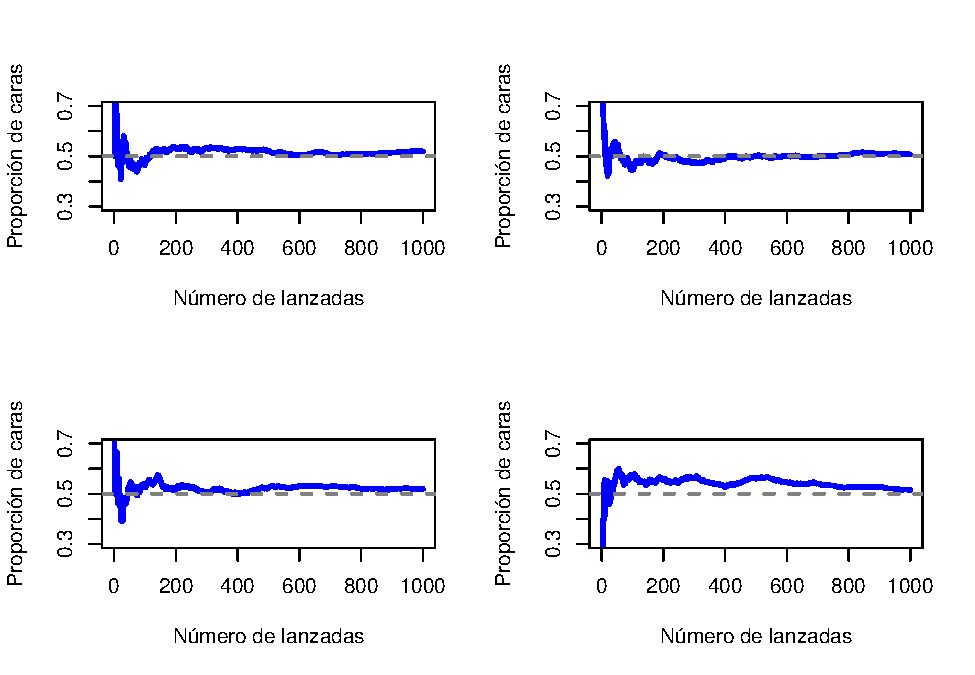
\includegraphics{FdI2_files/figure-latex/frequentistprobability-1.pdf}
\caption{\label{fig:frequentistprobability} Una imagen de cómo funciona la
probabilidad frecuentista. Si lanzas una moneda justa una y otra vez, la
proporción de caras deja de fluctuar y converge hacia la probabilidad
real de 0.5. Cada panel muestra uno de las cuatro simulaciones con 1.000
lanzamientos cada uno. Aunque ninguna de estas simulaciones terminó con
un valor exacto de .5, si hubiéramos extendido el experimento por un
número infinito de lanzamientos lo habríamos conseguido.}
\end{figure}

La definición frecuentista de probabilidad tiene algunas características
que le hacen deseable. En primer lugar, es objetivo: la probabilidad de
un evento se basa \emph{necesariamente} en el mundo real. La única forma
en que declaraciones de probabilidad puedan tener sentido es si se
refieren a (una secuencia de) eventos que ocurren en el universo físico.
En segundo lugar, es inequívoco: dos personas que miran como se
desarrolla la misma secuencia de eventos, al tratar de calcular la
probabilidad de un evento, inevitablemente deberán llegar a la misma
respuesta. Sin embargo, también tiene algunas características no tan
deseables. En primer lugar, no existen secuencias infinitas en el mundo
físico. Supongamos que has encontrado una moneda en el suelo y has
comenzado a lanzarla varias veces. Cada vez que aterriza, impacta en el
suelo. Cada impacto daña un poco la moneda; eventualmente, la moneda
será inutilizable. Entonces, uno podría preguntarse si realmente tiene
sentido fingir que una secuencia ``infinita'' de lanzamientos de monedas
es un concepto significativo u objetivo. No podemos decir que una
``secuencia infinita'' de eventos es algo real en el universo físico,
porque el universo físico no permite nada infinito. Así, podemos ver que
la definición frecuentista tiene un alcance limitado. Hay muchas cosas
por ahí a las que los seres humanos estamos felices de asignar
probabilidades en el día a día, pero que no pueden (ni siquiera en
teoría) ser planteadas como una secuencia hipotética de eventos. Por
ejemplo, si un meteorólogo aparece en televisión y dice: ``la
probabilidad de lluvia en Pamplona el 2 de noviembre del 2048 es del
60\%'' nosotros podemos aceptarlo sin rechistar. Pero desde un punto de
vista frecuentista, no queda tan claro cómo podemos definirlo. Sólo hay
una ciudad de Pamplona (en Navarra), y sólo un 2 de noviembre del 2048.
Aquí no hay una secuencia infinita de eventos, solo una cosa de una vez.
La probabilidad frecuentista nos \emph{prohíbe} hacer declaraciones de
probabilidad sobre un solo evento. Desde la perspectiva frecuentista,
lloverá mañana o o no lloverá; no hay una ``probabilidad'' que se pueda
adjuntar a un sólo evento no repetible. Sin embargo, existen algunos
trucos que los frecuentistas pueden utilizar para solucionar esta
situación. Una posibilidad es que el meteorólogo en realidad nos quiera
decir algo así: ``Existe una categoría de días para la que predigo un
60\% probabilidad de lluvia; si miramos sólo esos días para los que hago
esta predicción, entonces en el 60\% de esos días lloverá realmente''.
Es un poco extraño y contradictorio pensarlo de esta manera, pero los
frecuentistas hacen esto a veces.

\subsection{La visión bayesiana}\label{la-vision-bayesiana}

La alternativa a la visión frecuentista, la \textbf{\emph{visión
bayesiana}} de la probabilidad, a menudo se denomina visión
subjetivista, y es una visión relativamente minoritaria entre los
estadísticos, aunque ha ido ganando terreno constantemente a lo largo de
las últimas décadas. Hay muchos formas de bayesianismo, lo que hace
difícil decir exactamente cuál es ``la'' visión bayesiana. La forma más
fácil de entender la probabilidad subjetiva es al definir la
probabilidad de un evento como el \textbf{\emph{grado de creencia}} que
un agente inteligente y racional asigna a la verdad de ese evento. Desde
esa perspectiva, las probabilidades no existen en el mundo, sino más
bien en los pensamientos y suposiciones de las personas y otros seres
inteligentes. Sin embargo, para que este enfoque funcione, necesitamos
una forma de operacionalizar este ``grado de creencia''. Una forma de
hacerlo es formalizándolo en términos de una ``apuesta racional'' aunque
existen muchas otras formas. Supongamos que creo que existe una
probabilidad de que llueva mañana de un 60\%. Si alguien me hace una
apuesta, si llueve mañana, gano \$5, pero si no llueve, pierdo \$5.
Claramente, desde mi punto de vista, esta es una buena apuesta. Por otro
lado, si creo que la probabilidad de lluvia es sólo del 40\%, entonces
es una mala apuesta. Por lo tanto, podemos poner en práctica la noción
de una ``probabilidad subjetiva'' en términos de qué apuestas que estoy
dispuesto a aceptar.

¿Cuáles son las ventajas y desventajas del enfoque bayesiano? La
principal ventaja es que le permite asignar probabilidades a cualquier
evento. No esta limitado a aquellos eventos que son repetibles. La
principal desventaja (para muchas personas) es que no podemos ser
realmente objetivos - especificar una probabilidad requiere que
especifiquemos la entidad que tiene el grado de creencia que estamos
examinando. Esta entidad puede ser un humano, un extraterrestre, un
robot o incluso un estadístico, pero tiene que ser un agente inteligente
que sea capaz de creer en cosas. Para muchas personas esto representa un
inconveniente: parece hacer que la probabilidad sea arbitraria. Si bien
el enfoque bayesiano requiere que el agente en cuestión sea racional (es
decir, que obedezca las reglas de la probabilidad), permite que todos
tengan sus propias creencias; yo puedo creer que la moneda es justa
mientras que otro no, aunque ambos seamos racionales. La visión
frecuentista no permite que dos observadores atribuyan diferentes
probabilidades al mismo evento: cuando eso sucede, al menos uno de ellos
debe estar equivocado. La visión bayesiana no evita que esto ocurra. Dos
observadores con diferentes conocimientos previos pueden tener creencias
diferentes sobre el mismo evento. En otras palabras, mientras que la
visión frecuentista se puede considerar como demasiado estrecha (prohíbe
muchas cosas a las cuales queremos asignar probabilidades), la visión
bayesiana puede resultar demasiado amplia (permite demasiadas
diferencias entre observadores).

\subsection{¿Cuál es la diferencia? ¿Y quién tiene
razón?}\label{cual-es-la-diferencia-y-quien-tiene-razon}

Ahora que hemos visto ambas visiones estadísticas de forma
independiente, es necesario compararlas. Regresemos al hipotético juego
de fútbol de robots que comentamos comienzo del tema. ¿Que dirían un
frecuentista y un bayesiano sobre las tres afirmaciones? ¿Qué enunciado
sería la definición de probabilidad correcta para el frecuentista? ¿Y
para el bayesiano? ¿Es posible que alguno de los enunciados no tenga
sentido para cualquiera de los dos? Si entendemos ambas perspectivas,
podemos intuir cómo responder a estas preguntas.

Entendiendo las diferencias, podemos preguntarnos a continuación cuál de
dos enfoques es el \emph{correcto}. Sin embargo, no existe una respuesta
correcta. Matemáticamente hablando, no hay nada incorrecto sobre la
forma en que los frecuentistas piensan sobre secuencias de eventos, ni
hay nada incorrecto acerca de la forma en que los bayesianos definen las
creencias de un agente racional. De hecho, si vamos al detalle, los
bayesianos y los frecuentistas en realidad están de acuerdo en muchas
cosas. Muchos métodos frecuentistas conducen a decisiones que los
bayesianos pensarían que toma un agente racional. Muchos métodos
bayesianos tienen buenas propiedades frecuentistas.

En cualquier caso, la mayor parte de los métodos y análisis estadísticos
en la literatura se basan en el enfoque frecuentista. Por lo tanto, el
objetivo de esta asignatura es cubrir aproximadamente el mismo temario
que una clase típica de estadística de pregrado en ciencias de la
educación, y si queremos entender las herramientas estadísticas
utilizadas por la mayoría de los educadores en investigación,
necesitaremos una buena comprensión de los métodos frecuentistas.

\section{Teoría de probabilidad básica}\label{basicprobability}

A pesar de los argumentos ideológicos entre bayesianos y frecuentistas,
existe un consenso más o menos generalizado sobre las reglas que la
probabilidad debe obedecer. Hay muchas formas de abordar estas reglas.
El enfoque más utilizado se basa en el trabajo de Andrey Kolmogorov, uno
de los grandes matemáticos soviéticos del siglo XX. No entraremos mucho
en detalle, pero aprenderemos en qué consisten y cómo utilizarlas a
través del siguiente ejemplo.

\subsection{Introducción a las distribuciones de
probabilidad}\label{introduccion-a-las-distribuciones-de-probabilidad}

Un hecho comprobado sobre mi vida es que sólo tengo 5 pares de
pantalones: tres pares de vaqueros, los pantalones de un traje y un par
de pantalones de chándal. Lo más triste es que les he dado nombres: los
llamo \(X_1\), \(X_2\), \(X_3\), \(X_4\) y \(X_5\). Diariamente, por la
mañana, elijo un único par de esos pantalones que voy a usar. Si yo
tuviera que describir esta situación usando el lenguaje de la teoría de
la probabilidad, me referiría a cada par de pantalones (es decir, a cada
\(X\)) como un \textbf{\emph{evento elemental}}. La característica clave
de estos eventos elementales es que cada vez que hacemos una observación
(por ejemplo, cada vez que escojo un par de pantalones), el resultado
será uno y solo uno de estos eventos. Como he dicho antes, siempre uso
exactamente sólo un par de pantalones, así que mis pantalones cumplen
con esta restricción. Del mismo modo, al conjunto de todos los eventos
posibles se le denomina \textbf{\emph{espacio muestral}}. Siguiendo con
el ejemplo, mi espacio muestral sería el armario que contiene los 5
pantalones.

Bien, ahora que tenemos un espacio muestral (un armario), que está
construido a partir de muchas posibles eventos elementales (pantalones),
lo que queremos hacer es asignar una \textbf{\emph{probabilidad}} a cada
uno de estos eventos elementales. Para un evento \(X\), la probabilidad
de ese evento \(P(X)\) es un número que se encuentra entre 0 y 1. Cuanto
mayor sea el valor de \(P(X)\), más probable será que ocurra el evento.
Entonces, por ejemplo, si \(P(X) = 0\), significa que el evento \(X\) es
imposible (es decir, nunca uso esos pantalones). Por otro lado, si
\(P(X) = 1\) significa que el evento \(X\) es seguro que ocurra (es
decir, siempre uso esos pantalones). Los valores de probabilidad
intermedios, significan que a veces uso esos pantalones (y a veces no).
Por ejemplo, una \(P(X) = 0.5\) significa que uso esos pantalones la
mitad de las veces.

Llegados a este punto, lo siguiente que debemos entender es que ``algo
siempre sucede''. Cada vez que me pongo unos pantalones, realmente
termino usando esos pantalones. Lo que esto significa en términos
probabilísticos, es que las probabilidades de todos los eventos
elementales siempre suman 1. Esto se conoce como la \textbf{\emph{ley de
probabilidad total}}. Si se cumplen estos requisitos (tenemos número
\(X\) de pantalones, cada par con una probabilidad \(P(X)\) de usarlos
que en total suman 1), entonces lo que tenemos es una
\textbf{\emph{distribución de probabilidad}}.Veamos un ejemplo de
distribución de probabilidad

\begin{longtable}[]{@{}llllll@{}}
\toprule
Pantalones & V..azules & V..grises & V..negros & Traje.negro &
Chándal.azul\tabularnewline
\midrule
\endhead
Nombre & \(X_1\) & \(X_2\) & \(X_3\) & \(X_4\) & \(X_5\)\tabularnewline
Probabilidad & \(P(X_1) = .5\) & \(P(X_2) = .3\) & \(P(X_3) = .1\) &
\(P(X_4) = 0\) & \(P(X_5) = .1\)\tabularnewline
\bottomrule
\end{longtable}

Cada uno de estos eventos tiene una probabilidad que se encuentra entre
0 y 1, y si sumamos la probabilidad de todos eventos, suman 1. Incluso
podemos dibujar un gráfico de barras para visualizar esta distribución,
como se muestra en la Figura \ref{fig:pantsprob}.

\begin{figure}
\centering
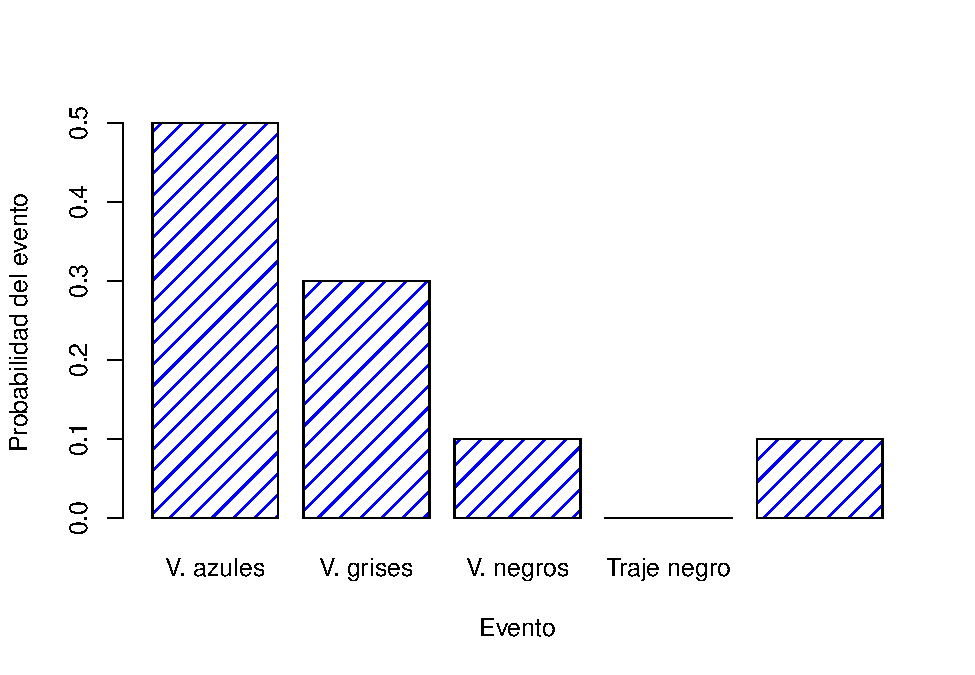
\includegraphics{FdI2_files/figure-latex/pantsprob-1.pdf}
\caption{\label{fig:pantsprob}Demostración visual de la distribución de
probabilidad de los ``pantalones''. Existen 5 ``eventos elementales'',
que se corresponden con mis 5 pares de pantalones. Cada evento tiene una
probabilidad de ocurrir: esta probabilidad es un número entre 0 y 1. La
suma de estas probabilidades es 1.}
\end{figure}

Es importante señalar que la teoría de probabilidades permite hablar
acerca de eventos elementales pero también sobre los
\textbf{\emph{eventos no elementales}}. La forma más fácil de ilustrar
este concepto es con un ejemplo. Siguiendo con el ejemplo de los
pantalones, es perfectamente posible hablar sobre la probabilidad de
usar vaqueros. Bajo esta premisa, podemos decir que el evento ``yo uso
vaqueros'' es posible siempre y cuando ocurra alguno de los eventos
elementales apropiados; en este caso ``vaqueros azules'', ``vaqueros
negros'' o ``vaqueros grises''. En términos matemáticos, definimos al
evento \(E\) ``vaqueros'' como el conjunto de eventos elementales
\((X_1, X_2, X_3)\). Si se produce alguno de estos eventos elementales,
también podemos decir que \(E\) ha ocurrido. Por lo tanto, podemos decir
que la probabilidad \(P(E)\) es simplemente la suma de esos tres
eventos, así \[
P(E) = P(X_1) + P(X_2) + P(X_3)
\] y, dado que las probabilidades de los vaqueros azules, grises y
negros son respectivamente .5, .3 y .1, la probabilidad total de usar
vaqueros es igual a .9.

Todo esto parece obvio y simple. Sin embargo, a partir de estos simples
comienzos, es posible construir algunas herramientas matemáticas más
complejas y poderosas. En la siguiente Tabla se muestran algunas de las
otras reglas que deben de cumplirse para poder calcular probabilidades.

\begin{longtable}[]{@{}llll@{}}
\toprule
Castellano & Notacion & Igual & Formula\tabularnewline
\midrule
\endhead
No \(A\) & \(P(\neg A)\) & = & \(1-P(A)\)\tabularnewline
\(A\) o \(B\) & \(P(A \cup B)\) & = &
\(P(A) + P(B) - P(A \cap B)\)\tabularnewline
\(A\) y \(B\) & \(P(A \cap B)\) & = &
\(P(A \vert B) P(B)\)\tabularnewline
\bottomrule
\end{longtable}

\section{La distribución binomial}\label{binomial}

Como hemos visto, las distribuciones de probabilidad pueden variar
enormemente, por lo que existe un gran número de distribuciones
posibles. Sin embargo, no todas son igual de importantes. Las
distribuciones más importantes, y de las que hablaremos en esta
asignatura son cinco: la distribución binomial, la distribución normal,
la distribución \(t\), la distribución \(\chi^2\) (``chi-cuadrada'') y
la distribución \(F\). Daremos una breve introducción a las cinco,
prestando especial atención a las distribuciones binomial y normal.
Comenzaremos con la distribución más simple de las cinco, la
distribución binomial.

\subsection{Introducción al binomio}\label{introduccion-al-binomio}

La teoría de la probabilidad se creó originalmente para intentar
describir cómo funcionaban los juegos de azar, por lo que parece
adecuado que nuestra discusión sobre la \textbf{\emph{distribución
binomial}} involucre una discusión sobre tirar dados y lanzar monedas.
Imaginemos el siguiente ``experimento'': tengo en mi poder 20 dados
iguales de seis caras. En una de las caras de cada dado hay una imagen
de una calavera; las otras cinco caras están en blanco. Si tiro los 20
dados, ¿cuál es la probabilidad de que obtenga exactamente 4 calaveras?
Asumiendo que los dados son justos, sabemos que la probabilidad de que
en un dado salga la calavera es de de 1 en 6; dicho de otra forma, la
probabilidad de que salga calavera en un solo dado es de aproximadamente
\(.167\). Esta información es suficiente para poder responder a nuestra
pregunta anterior, así que veamos cómo hacerlo.

Primero, pondremos algunos nombres a los eventos con su respectiva
notación. Dejaremos que \(N\) denote el número de dados que se tiran en
nuestro experimento; a esto se le conoce como el \textbf{\emph{parámetro
de tamaño}} de nuestra distribución binomial. También usaremos
\(\theta\) para referirnos a la probabilidad de que al tirar un solo
dado salga calavera, una cantidad que generalmente se denomina como la
\textbf{\emph{probabilidad de éxito}} del binomio.\footnote{Hay que
  tener en cuenta que el término ``éxito'' es bastante arbitrario, y en
  realidad no implica que el resultado sea algo deseado. Si \(\theta\)
  se refiriera a la probabilidad de que un pasajero se lesione en un
  accidente de autobús, seguiría siendo una probabilidad de éxito,
  aunque en realidad no queremos que la gente salga lastimada}
Finalmente, usaremos \(X\) para referirnos a los resultados de nuestro
experimento, es decir, la cantidad de calaveras que obtengo cuando lanzo
los dados. Dado que el valor real de \(X\) se debe al azar, nos podemos
referir a ella como una \textbf{\emph{variable aleatoria}}. En cualquier
caso, ahora que tenemos toda esta terminología y notación, podemos
utilizarlos para exponer el problema que planteábamos en el párrafo
anterior con mayor precisión. La cantidad que queremos calcular es la
probabilidad de que \(X = 4\) sabiendo que \(\theta = .167\) y \(N=20\).
La ``forma'' general de esta probabilidad que me interesa calcular
podría escribirse como, \[
  P(X \ | \ \theta, N)
\] donde estamos interesados en el caso específico donde \(X=4\),
\(\theta = .167\) y \(N=20\). Hace falta un elemento de notación más
antes de continuar con la solución del problema. Si yo quiero decir que
\(X\) se genera aleatoriamente a partir de una distribución binomial con
los parámetros \(\theta\) y \(N\), la notación que usaría para
expresarlo sería la siguiente: \[
  X \sim \mbox{Binomial}(\theta, N)
\]

Aunque no utilizaremos las fórmulas para hacer cálculos formalmente,
dejaré la fórmula de la distribución binomial en la Tabla
\ref{tab:distformulas}, ya que puede ser útil si se quieren entender
temas más avanzados con algo de profundidad. Por lo pronto, analizaremos
como se ve una distribución binomial (puedes hacerlo tú mismo si entras
aquí{[}\url{https://leudave.shinyapps.io/distribuciones/}{]}). La Figura
\ref{fig:binomial1} dibuja la probabilidad binomial para todos los
valores posibles de \(X\) de nuestro experimento de lanzamiento de
dados, partiendo desde \(X=0\) (ninguna sale calavera) hasta \(X=20\)
(salen todas calaveras). Hay que tener en cuenta que esto es básicamente
un gráfico de barras, al igual que la gráfica de la ``probabilidad de
pantalones'' de la Figura \ref{fig:pantsprob}. En el eje horizontal
tenemos todos los eventos posibles, y en el eje vertical podemos leer la
probabilidad de que ocurra cada uno de esos eventos. Por lo tanto, la
probabilidad de que salgan 4 calaveras al tirar 20 dados es de
aproximadamente 0,20 (la respuesta exacta es 0,2022036, como veremos en
un momento). En otras palabras, esperaría que ese evento suceda
aproximadamente el 20\% de las veces que se lleve a cabo este
experimento.

\begin{table}[t]

\caption{\label{tab:distformulas}Fórmulas para las distribuciones binomial y normal. En la ecuación de la binomial, $X!$ es una función factorial (es decir, multiplica todos los números enteros de  1 hasta $X$), y en la de la distribución normal "exp" se refiere a una función exponencial.}
\centering
\begin{tabular}{l|l}
\hline
Binomial & Normal\\
\hline
\$P(X | \textbackslash{}theta, N) = \textbackslash{}displaystyle\textbackslash{}frac\{N!\}\{X! (N-X)!\}  \textbackslash{}theta\textasciicircum{}X (1-\textbackslash{}theta)\textasciicircum{}\{N-X\}\$ & \$p(X | \textbackslash{}mu, \textbackslash{}sigma) = \textbackslash{}displaystyle\textbackslash{}frac\{1\}\{\textbackslash{}sqrt\{2\textbackslash{}pi\}\textbackslash{}sigma\} \textbackslash{}exp \textbackslash{}left( -\textbackslash{}frac\{(X - \textbackslash{}mu)\textasciicircum{}2\}\{2\textbackslash{}sigma\textasciicircum{}2\} \textbackslash{}right)\$\\
\hline
\end{tabular}
\end{table}

\begin{figure}
\centering
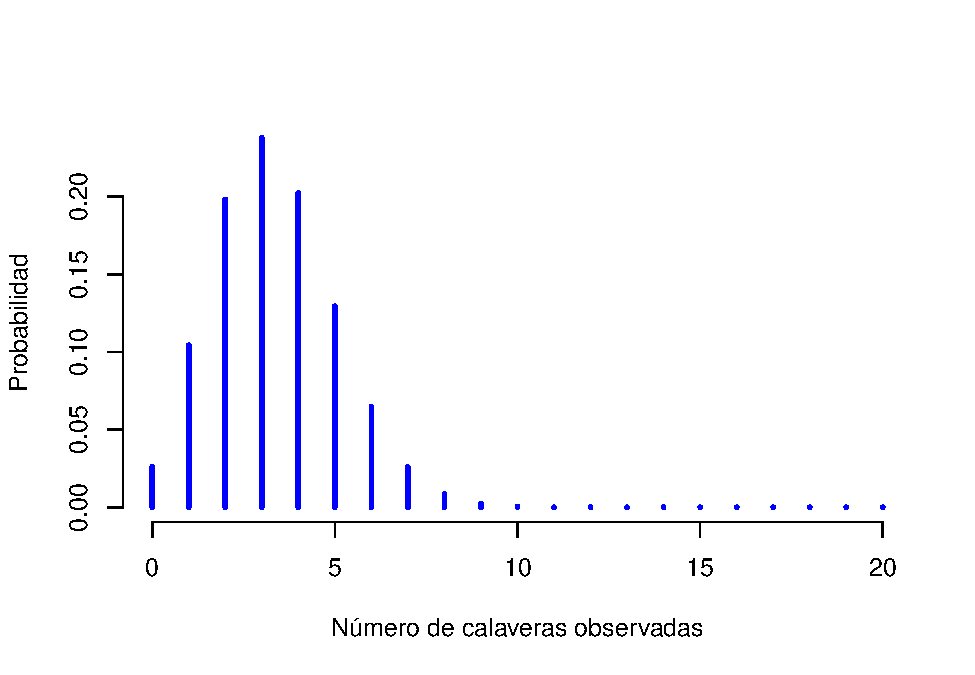
\includegraphics{FdI2_files/figure-latex/binomial1-1.pdf}
\caption{\label{fig:binomial1} La distribución binomial con parámetro de
tamaño de \(N=20\) y una probabilidad de éxito de \(theta = 1/6\). Cada
barra vertical representa la probabilidad de un resultado específico (un
valor posible de \(X\)). Ya que esta es una distribución de
probabilidad, cada una de las probabilidades debe ser un número entre 0
y 1, y la altura de las barras también deben sumar 1.}
\end{figure}

Para darte una idea de cómo cambia la distribución binomial cuando
modificamos los valores de \(\theta\) y \(N\), supongamos que en lugar
de tirar dados, en realidad estoy lanzando monedas. Esta vez, mi
experimento implica lanzar una moneda justa repetidamente, y el
resultado que me interesa es la cantidad de caras que observo. En este
escenario, la probabilidad de éxito ahora es de \(\theta = 1/2\).
Supongamos que tirara la moneda \(N=20\) veces. En este ejemplo, he
cambiado la probabilidad de éxito, pero mantuve el tamaño de la muestra
del experimento. ¿Qué efecto tiene este cambio en nuestra distribución
binomial? Bueno, como la Figura \ref{fig:binomial2a} muestra, el efecto
principal fue el desplazamiento de toda la distribución hacia la
derecha, como era de esperar. ¿Y si lanzamos una moneda \(N=100\) veces?
En este caso obtendremos algo como lo de la Figura \ref{fig:binomial2b}.
La distribución se mantiene aproximadamente en el medio, pero hay un
poco más de variabilidad en los posibles resultados.

\begin{figure}
\centering
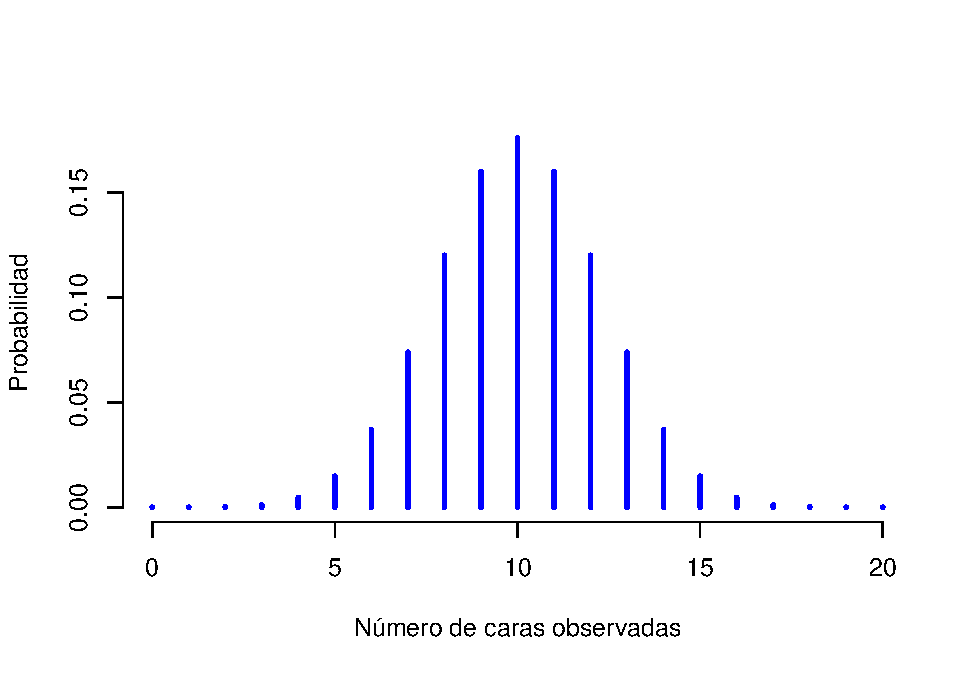
\includegraphics{FdI2_files/figure-latex/binomial2a-1.pdf}
\caption{\label{fig:binomial2a}Dos distribuciones binomiales, que involucran
un escenario en el que lanzo una moneda justa, donde la probabilidad de
éxito es \(theta = 1/2\). Asumimos que estoy lanzando la moneda \(N=20\)
veces.}
\end{figure}

\begin{figure}
\centering
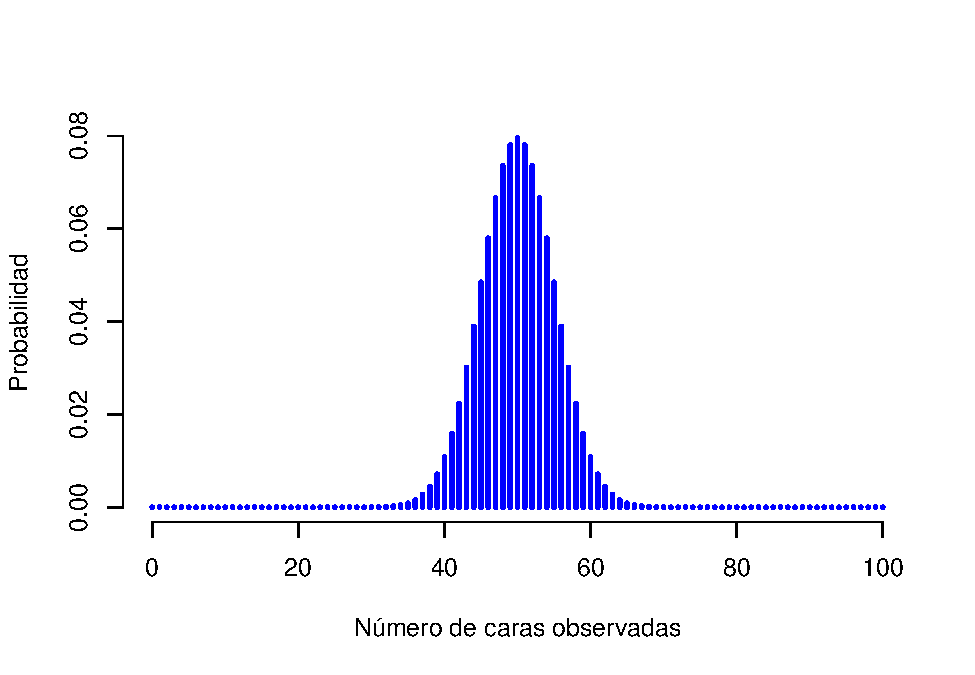
\includegraphics{FdI2_files/figure-latex/binomial2b-1.pdf}
\caption{\label{fig:binomial2b}Dos distribuciones binomiales, que involucran
un escenario en el lanzo una moneda justa, donde la probabilidad de
éxito subyacente es \(theta = 1/2\). Asumimos que estoy lanzando la
moneda \(N=100\) veces.}
\end{figure}

\section{La distribución normal}\label{normal}

Si bien la distribución binomial es conceptualmente la distribución más
sencilla de entender, no es la más importante. Ese honor le corresponde
a la \textbf{\emph{distribución normal}}, también conocida como ``curva
de campana'' o como ``distribución gaussiana'' o ``campana de Gauss''.
Una distribución normal se describe utilizando dos parámetros, la media
de la distribución \(\mu\) y la desviación estándar de la distribución
\(\sigma\). La notación que utilizamos para decir que una variable \(X\)
se distribuye normalmente es la siguiente:

\[
  X \sim \mbox{Normal}(\mu,\sigma)
\] Al igual que con la distribución binomial, he incluido la fórmula
para la distribución normal en la tabla \ref{tab:distformulas}, porque
creo que es lo suficientemente importante como para que todos los que
aprenden algo de estadística al menos la conozcan, aunque no nos
enfoquemos en ella.

Vamos intentar descifrar lo que significa que una variable esté
normalmente distribuida. Echemos un vistazo a la Figura
\ref{fig:normdist}, que muestra una distribución normal con media
\(\mu = 0\) y desviación estándar \(\sigma = 1\). Con un poco de
imaginación, podemos apreciar de dónde viene el nombre ``curva de
campana''. A diferencia de los gráficos sobre la distribución binomial,
la imagen de la distribución normal en la Figura \ref{fig:normdist}
muestra una curva suave en lugar de barras ``tipo histograma''. Esto no
es arbitrario: la distribución normal es continua, mientras que la
distribución binomial es discreta. Por ejemplo, en el experimento de
tiro de dados de la sección anterior, es posible obtener 3 calaveras o 4
calaveras, mientras que un valor intermedio como 3.9 es imposible de
obtener. Este hecho se ve reflejado en la Figura \ref{fig:binomial1},
donde tenemos una barra ubicada en \(X=3\) y otra en \(X=4\), pero entre
ellas no hay nada. En cambio, los valores continuos no tienen esta
restricción. Por ejemplo, supongamos que estamos hablando del tiempo. La
temperatura de un día primavera podría ser de 23 grados, 24 grados, 23.9
grados o cualquier cosa intermedia, ya que la temperatura es una
variable continua, por lo que una distribución normal podría ser la
herramienta apropiada para describir las diferentes temperaturas en los
días de primavera.\footnote{En la práctica, la distribución normal es
  tan útil que las personas tienden a usarla incluso cuando la variable
  no es continua. Siempre que haya suficientes categorías (por ejemplo,
  respuestas de escala Likert de un cuestionario), suele ser frecuente
  el uso de la distribución normal.}

\begin{figure}
\centering
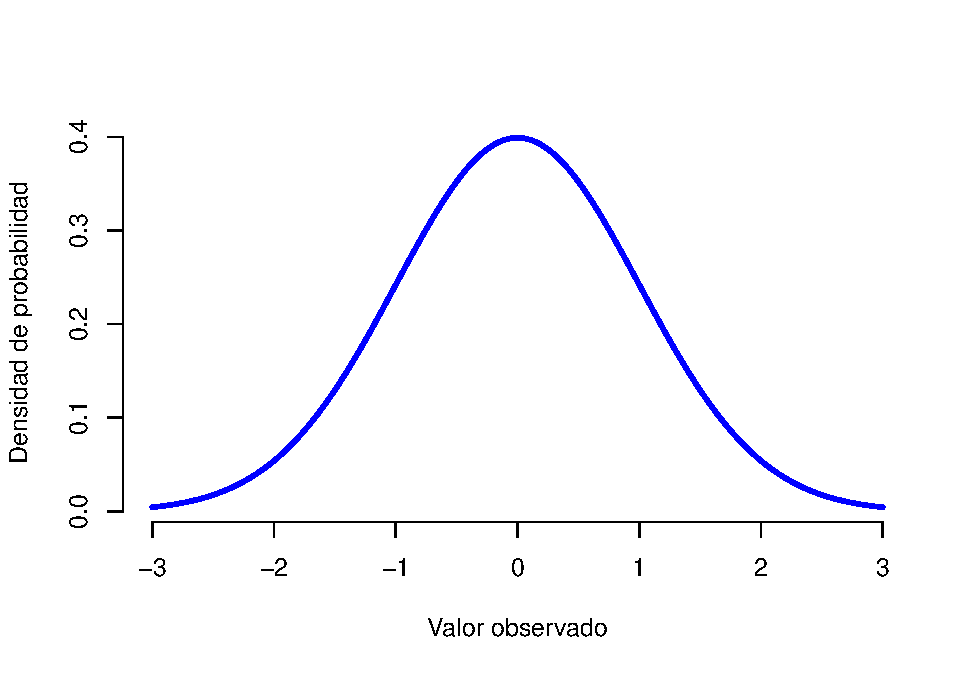
\includegraphics{FdI2_files/figure-latex/normdist-1.pdf}
\caption{\label{fig:normdist} Distribución normal con media \(mu = 0\) y
desviación estándar \(sigma = 1\). El eje \(x\) corresponde con el valor
de alguna variable, y el eje \(y\) nos dice qué tan probable es que
observemos ese valor. Sin embargo, vemos como el eje \(y\) se denomina
``Densidad de Probabilidad'' y no ``Probabilidad''. La altura de la
curva no representa como tal la probabilidad de observar un valor
particular de \(x\). Sin embargo, las alturas nos informan sobre qué
valores de \(x\) son más probables (¡los más altos!).}
\end{figure}

Una vez visto esto, vamos a analizar cómo funciona una distribución
normal. En primer lugar, veamos qué es lo que sucede cuando jugamos con
los parámetros de la distribución (puedes hacerlo tú mismo si entras en
este enlace). La Figura \ref{fig:normmean} muestra distribuciones
normales que tienen medias diferentes, pero con la misma desviación
estándar. Como es de esperar, todas estas distribuciones tienen la misma
``anchura''. La unica diferencia entre ellas es que se han desplazado
hacia la izquierda o hacia la derecha. En todos los demás aspectos son
idénticas. Por el contrario, si aumentamos la desviación estándar
mientras mantenemos la media constante, el pico de la distribución
permanece en el mismo lugar, pero la distribución se amplía, como
podemos ver en la Figura \ref{fig:normsd}. Sin embargo, cuando ampliamos
la distribución, la altura del pico disminuye. Esto \emph{tiene} que
suceder: de la misma forma que las alturas de las barras de una
distribución binomial discreta tienen que \emph{sumar} 1, el total del
\emph{área bajo la curva} de una distribución normal debe ser igual a 1.

\begin{figure}
\centering
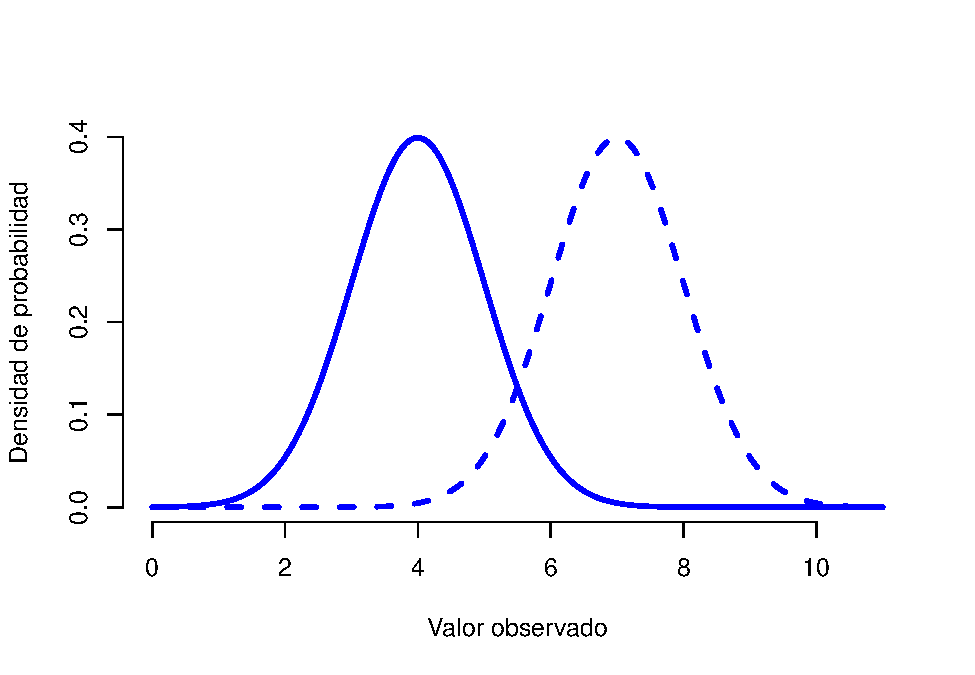
\includegraphics{FdI2_files/figure-latex/normmean-1.pdf}
\caption{\label{fig:normmean}Gráfica que demuestra lo que sucede cuando se
cambia la media de una distribución normal. La línea sólida representa
una distribución normal con media de \(mu=4\). La línea discontinua
muestra una distribución normal con una media de \(mu=7\). En ambos
casos, la desviación estándar es de \(sigma=1\). Vemos como las dos
distribuciones tienen la misma forma, pero la distribución con la línea
discontinua se desplaza hacia la derecha.}
\end{figure}

\begin{figure}
\centering
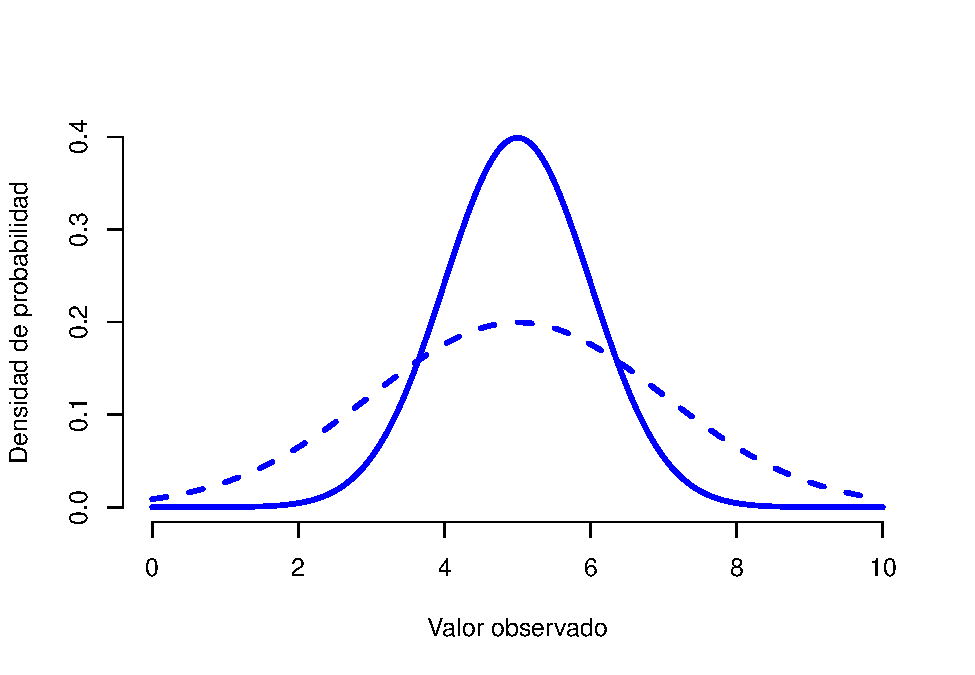
\includegraphics{FdI2_files/figure-latex/normsd-1.pdf}
\caption{\label{fig:normsd}Una ilustración de lo que sucede cuando cambia la
desviación estándar de una distribución normal. Ambas distribuciones
tienen una media de \(mu=5\), pero diferentes desviaciones estándar. La
línea continua dibuja una distribución con una desviación estándar
\(sigma=1\), y la línea discontinua muestra una distribución con
desviación estándar de \(sigma=2\). Como consecuencia, ambas
distribuciones están centradas en el mismo lugar, pero la distribución
con la línea discontinua es más ancha que la otra.}
\end{figure}

Antes de seguir adelante, quiero señalar una característica importante
de la distribución normal. Independientemente de los valores de la media
y la desviación estándar, un 68.3\% del área de la curva cae dentro de 1
desviación estándar sobre la media. Del mismo modo, el 95.4\% de la
distribución cae dentro de 2 desviaciones estándar sobre la media, y el
99.7\% de la distribución está dentro de 3 desviaciones estándar. Esta
idea se ilustra en las Figuras \ref{fig:sdnorm1} y \ref{fig:sdnorm2}.

\begin{figure}
\centering
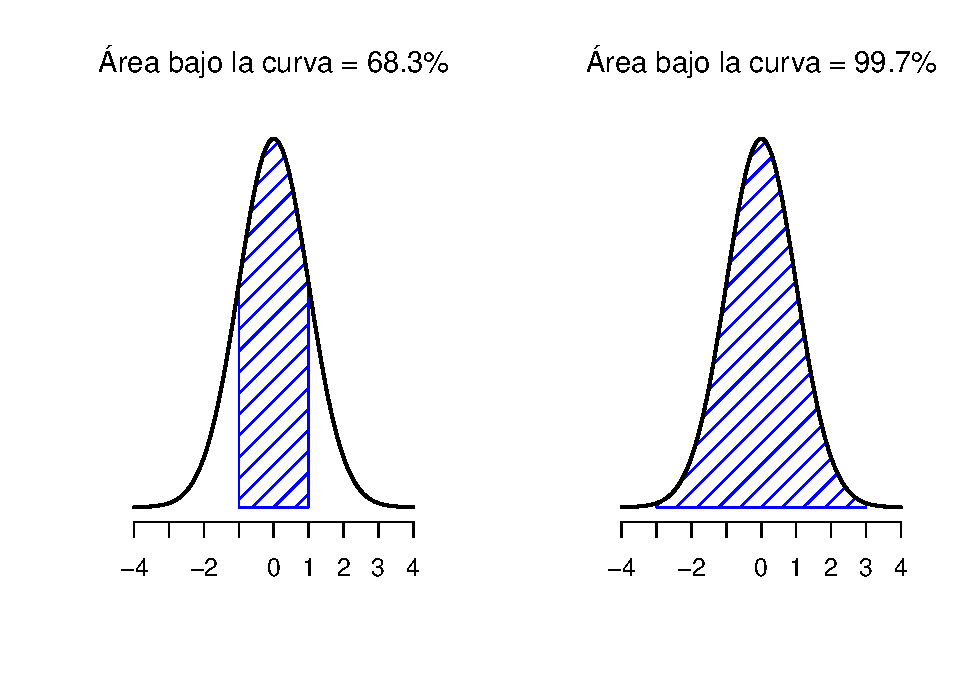
\includegraphics{FdI2_files/figure-latex/sdnorm1-1.pdf}
\caption{\label{fig:sdnorm1}El área bajo la curva indica la probabilidad de
que una observación se encuentre dentro de un rango determinado. Las
línea continua traza una distribución normal con media \(mu=0\) y
desviación estándar \(sigma=1\). El área sombreada ilustra el `área bajo
la curva' para dos casos importantes. En el panel a, podemos ver que hay
es un 68.3\% de probabilidad de que una observación caiga dentro de 1
desviación estándar sobre la media. En el panel b, vemos que existe una
probabilidad del 95.4\% de que una observación se encuentre dentro de 2
desviaciones estándar sobre la media.}
\end{figure}

\begin{figure}
\centering
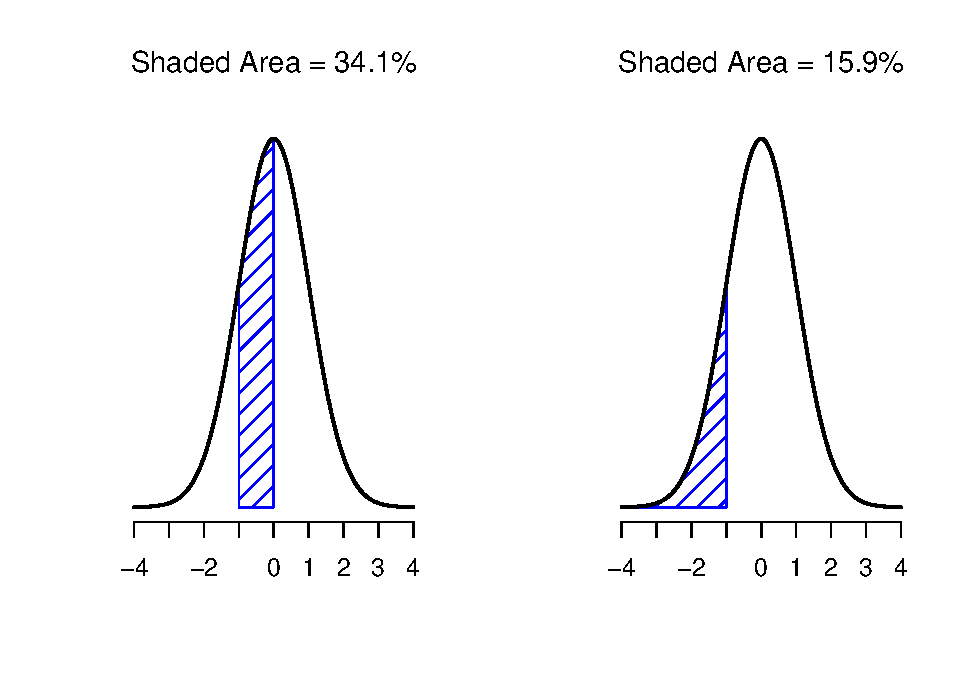
\includegraphics{FdI2_files/figure-latex/sdnorm2-1.pdf}
\caption{\label{fig:sdnorm2}Dos ejemplos más sobre el concepto del `área
bajo la curva'. Existe un 15.9\% de probabilidad de que una observación
se encuentre 1 desviación estándar o menos por debajo de la media (panel
a), y una probabilidad del 34.1\% de que una observación sea mayor que
una desviación estándar por debajo de la media pero menor que la media
(panel b). Si sumamos estos dos valores, obtendremos 15.9\% + 34.1\% =
50\%. Para datos que estén normalmente distribuidos, existe un 50\% de
probabilidad de que una observación caiga por debajo de la media. Esto
implica que existe un 50\% de probabilidad de que caiga por encima de la
media.}
\end{figure}

\subsection{Densidad de probabilidad}\label{density}

A lo largo de la discusión sobre la distribución normal, ha habido un
par de cosas que parecen no tener sentido. Quizás hayas notado que el
eje \(y\) en estas Figuras se denomina como ``Densidad de probabilidad''
en lugar de ``Probabilidad''. Tal vez notaste que utilizamos \(p(X)\) en
lugar de \(P(X)\) en la fórmula de la distribución normal.

Si utilizamos la Figura y calculamos (siguiendo la fórmula) la
probabilidad de \texttt{x\ =\ 1}, para una variable normalmente
distribuida con \texttt{media\ =\ 1} y desviación estándar
\texttt{sd\ =\ 0.1}, nos arrojará como resultado una probabilidad de
3.99.

Sin embargo, hemos visto anteriormente que las probabilidades \emph{no}
pueden ser mayores que 1. Entonces, ¿qué es lo que hemos calculado?

Lo que hemos calculado aquí en realidad no es una probabilidad: Para
entender qué es ese algo, tenemos que pensar qué es lo que realmente
\emph{significa} decir que \(X\) es una variable continua. Digamos que
estamos hablando de la temperatura otra vez. El termómetro me dice que
hacen 23 grados, pero yo sé que eso no es del todo cierto. No hacen 23
grados \emph{exactamente}. Quizás sea algo más cercano a los 23.1 grados
o, si seguimos, en realidad podrían ser 23.095 grados. Esto es lo que
sucede con los valores continuos: nunca se sabe el valor exacto.

Ahora pensemos en lo que esto implica cuando hablamos de probabilidades.
Supongamos la temperatura máxima para mañana se toma de una distribución
normal con media 23 y desviación estándar 1. ¿Cuál es la probabilidad de
que la temperatura sea \emph{exactamente} 23 grados? La respuesta es
``cero'', o posiblemente, ``un número tan cercano a cero que bien podría
ser cero''. ¿Por qué es esto? Es como intentar tirar un dardo en un
tablero de dardos con dianas infinitamente cada vez más pequeñas: no
importa cuán buena sea tu puntería, nunca acertarás. En la vida real
nunca obtendremos el valor exacto de 23. Siempre será 23.1 o 22.99998 o
algo así. En en otras palabras, no tiene sentido hablar de la
probabilidad de que la temperatura sea exactamente 23 grados. Sin
embargo, en el día a día, si el termómetro indica 23 grados pero en
realidad hacen 22.9998 grados, probablemente no nos importe demasiado.
Esto es porque en el día a día, ``23 grados'' por lo general significa
algo así como ``en algún lugar entre 22.5 y 23.5 grados''. Y aunque no
parezca muy importante preguntar por la probabilidad de que la
temperatura sea exactamente 23 grados, lo que sí lo parece es preguntar
sobre la probabilidad de que la temperatura se encuentre entre 22.5 y
23.5, o entre 20 y 30, o cualquier otro rango de temperaturas en el que
estemos interesados.

El objetivo de esta explicación es dejar claro que, cuando hablamos de
distribuciones continuas, no tiene sentido hablar sobre la probabilidad
de un valor específico. Sin embargo, sí que \emph{podemos} hablar sobre
la probabilidad de que el valor se encuentre dentro de un rango
particular de valores. Para encontrar probabilidad asociada con un rango
particular, lo que debe hacer es calcular el ``área bajo la curva''.
Este concepto lo conocemos: en la figura \ref{fig:sdnorm1}, las áreas
sombreadas representan probabilidades genuinas (por ejemplo, la Figura
\ref{fig:sdnorm1} muestra la probabilidad de observar un valor que cae
dentro de 1 desviación estándar sobre la media).

Para finalizar, volveremos con la fórmula para \(p(x)\) que vimos
anteriormente. Los resultados de \(p(x)\) no describe una probabilidad,
sino una \textbf{\emph{densidad de probabilidad}}, que en las gráficas
corresponde a la altura de la curva. De la misma forma en que las
probabilidades son números no-negativos que deben sumar 1, las
densidades de probabilidad son números no-negativos que deben integrar a
1 (donde la integral se toma a través de todos los valores posibles de
\(X\)). Para calcular la probabilidad de que \(X\) caiga entre \(a\) y
\(b\) calculamos la integral definida de la función de densidad sobre el
rango correspondiente, \(\int_a^b p(x) \ dx\). Se trata simplemente de
otra forma de llegar al mismo resultado.

\section{Otras distribuciones útiles}\label{otherdists}

La distribución normal es la distribución más utilizada por los
estadísticos (por razones que se discutirán más adelante), y la
distribución binomial es útil muchos escenarios. Sin embargo, existen
otros tipos de distribuciones de probabilidad. Revisaremos brevemente 3
de ellas: la distribución \(t\), la distribución \(\chi^2\) y la
distribución \(F\) - La \textbf{\emph{distribución \(t\)}} es una
distribución continua que se parece mucho a una distribución normal,
pero que tiene colas más pesadas (ver Figura) \ref{fig:tdist}. Esta
distribución tiende a surgir en situaciones en las que piensa que los
datos siguen una distribución normal, pero no se conoce la media o la
desviación estándar.

\begin{figure}
\centering
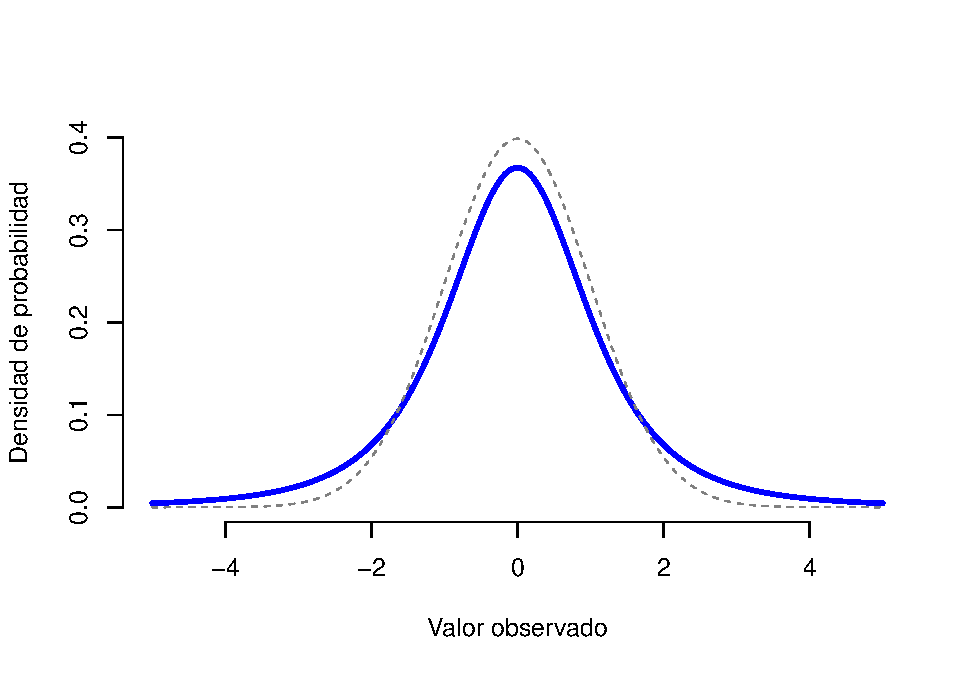
\includegraphics{FdI2_files/figure-latex/tdist-1.pdf}
\caption{\label{fig:tdist}Una distribución \(t\) con 3 grados de libertad
(línea continua). Se asemeja a una distribución normal, pero no es igual
(línea discontinua). Ten en cuenta que las ``colas'' de la distribución
\(t\) son más ``pesadas'' (es decir, se extienden más hacia afuera,
conteniendo más valores que se alejan de la media) que las colas de la
distribución normal.}
\end{figure}

\begin{itemize}
\tightlist
\item
  La \textbf{\emph{distribución \(\chi^2\)}} es otra distribución que
  podemos encontrar con cierta frecuencia. Es habitual encontrarla
  cuando hacemos análisis de datos categóricos. Los valores de una
  distribución \(\chi^2\) se consiguen al elevar al cuadrado los valores
  de una variable distribuída normalmente y luego sumarlos (un
  procedimiento denominado ``suma de cuadrados''). Después veremos
  porqué es útil hacer una ``suma de cuadrados''. La apariencia de una
  distribución \(\chi^2\) la puedes encontrar en la Figura
  \ref{fig:chisqdist}.
\end{itemize}

\begin{figure}
\centering
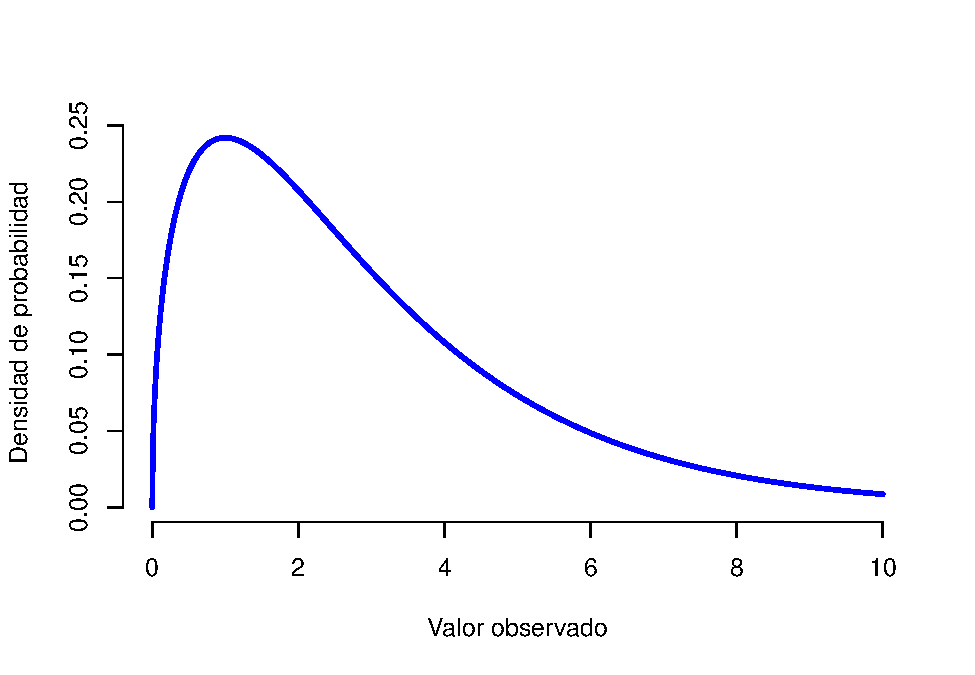
\includegraphics{FdI2_files/figure-latex/chisqdist-1.pdf}
\caption{\label{fig:chisqdist}Una distribución \(chi^2\) con 3 grados de
libertad (3 repeticiones, lo explicaremos más adelante). Observa que los
valores siempre deben ser mayores que cero (los valores se elevan al
cuadrado y se suman), y que la distribución es bastante sesgada (en este
caso hacia la derecha). Estas son las características clave de una
distribución chi-cuadrado.}
\end{figure}

\begin{itemize}
\tightlist
\item
  La \textbf{\emph{distribución \(F\)}} se parece un poco a la
  distribución \(\chi^2\) y surge cada vez que necesitamos comparar dos
  distribuciones \(\chi^2\) entre sí. Es decir, si queremos comparar dos
  ``sumas de cuadrados'' diferentes, nos encontraremos con una
  distribución \(F\). Aún no hemos visto un ejemplo de todo lo que
  implica una suma de cuadrados, pero lo veremos cuando hablemos sobre
  ANOVAs, donde nos encontraremos nuevamente con la distribución \(F\).
\end{itemize}

\begin{figure}
\centering
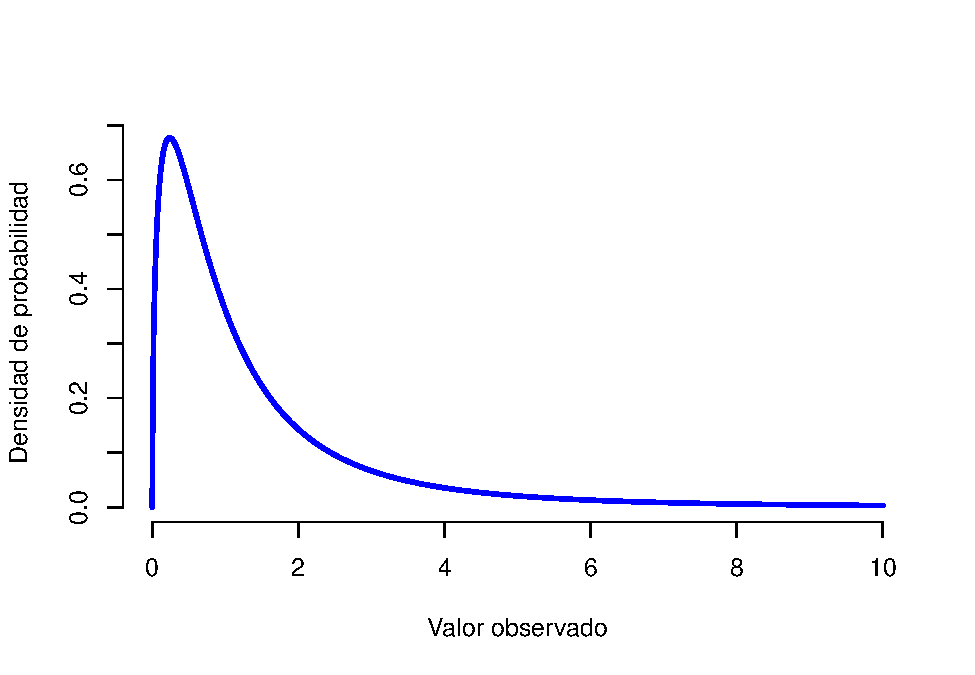
\includegraphics{FdI2_files/figure-latex/Fdist-1.pdf}
\caption{\label{fig:Fdist}Una distribución \(F\) con 3 y 5 grados de
libertad. Cualitativamente hablando, es similar a una distribución de
chi-cuadrado, pero por lo general el significado no es el mismo.}
\end{figure}

Debido a que estas distribuciones están estrechamente relacionadas con
la distribución normal y entre sí, y porque se convertirán en las
distribuciones importantes al hacer análisis estadísticos inferenciales
en este curso, creo que es útil hacer una pequeña demostración de cómo
estas distribuciones realmente están relacionadas entre sí. Primero,
imagina que tenemos un conjunto de 1,000 observaciones aleatorias
distribuidas normalmente al cual llamamos ``Muestra A''.

Por lo tanto, la ``Muestra A'' es una variable que contiene 1,000
números que se distribuyen normalmente, y tienen una media de 0 y
desviación estándar 1. En la Figura \ref{fig:distnormal} podemos ver un
histograma con la distribución de los valores organizados por columnas
así como una línea negra sólida que representa la distribución verdadera
de los datos (es decir, una distribución normal con media 0 y desviación
estándar 1. Así podemos comparar los datos recién generados con los de
una distribución normal verdadera.

\begin{figure}
\centering
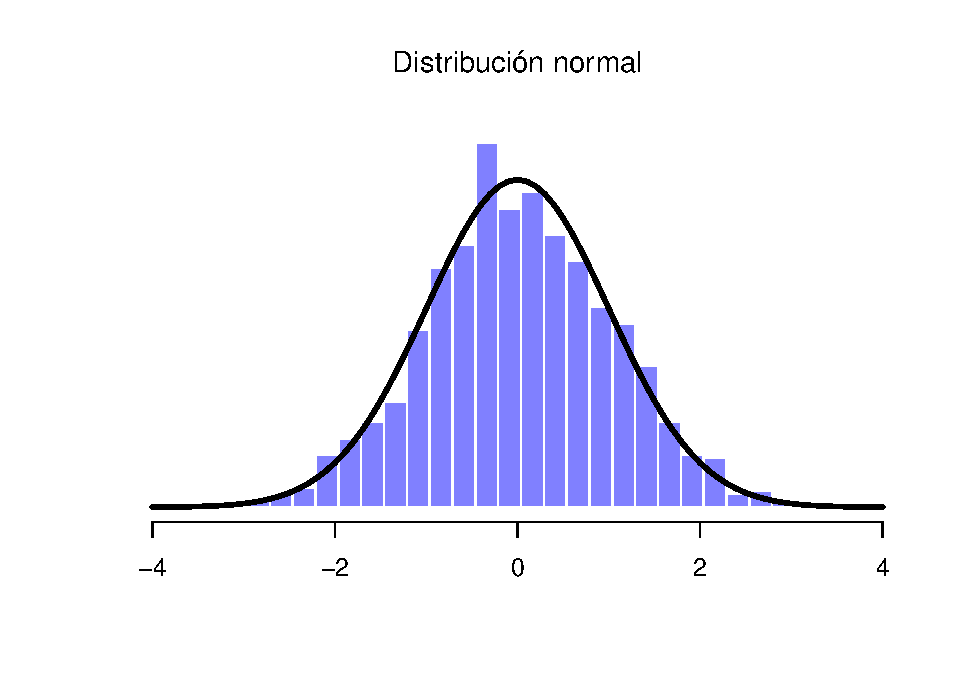
\includegraphics{FdI2_files/figure-latex/distnormal-1.pdf}
\caption{\label{fig:distnormal}Distribución normal de la Muestra A}
\end{figure}

En la Figura anterior podemos observar cómo han sido generados muchos
valores distribuidos normalmente que luego han sido comparados con la
distribución de probabilidad verdadera (línea sólida). Supongamos que
ahora queremos una distribución chi-cuadrada con 3 grados de libertad.
Como hemos mencionado anteriormente, una distribución chi-cuadrada con
\(k\) grados de libertad es es el resultado de tomar \(k\) variables
normalmente distribuidas (con media 0 y desviación estándar 1),
elevarlas al cuadrado y sumarlas. Como queremos una distribución de
chi-cuadrada con 3 grados de libertad, además de nuestra ``Muestra A'',
necesitamos dos conjuntos más de valores (también distribuidos
normalmente). A estas nuevas dos variables las llamaremos ``Muestra B''
y ``Muestra C'':

\begin{figure}
\centering
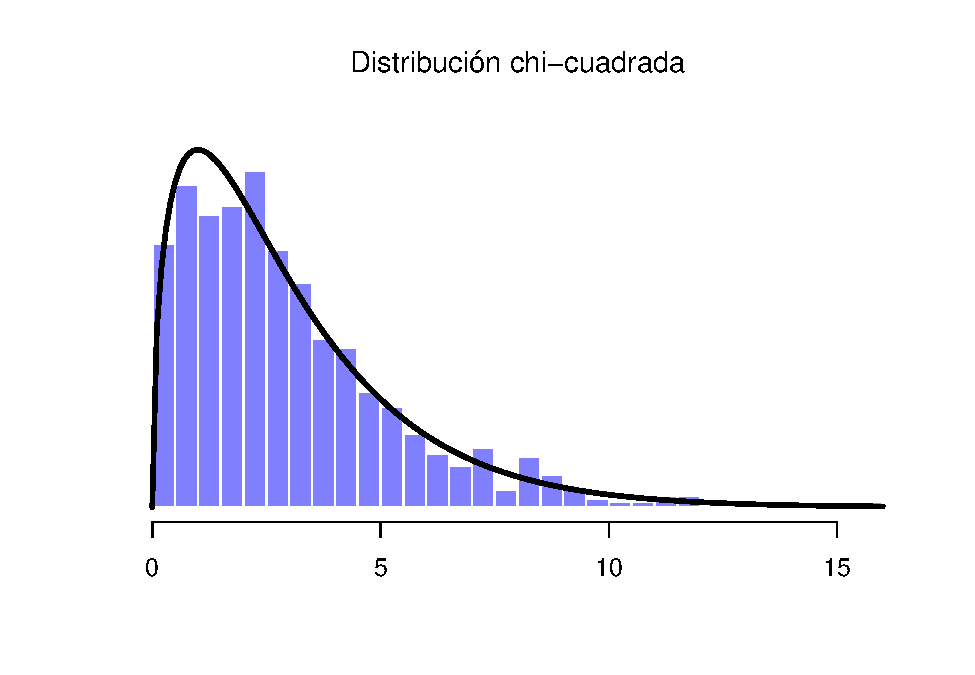
\includegraphics{FdI2_files/figure-latex/distchi-1.pdf}
\caption{\label{fig:distchi}Distribución chi-cuadrada. Incluye a las
Muestras A, B y C (3 grados de libertad)}
\end{figure}

Una vez que tenemos las tres variables, la teoría dice que debemos
elevarlos al cuadrado y sumarlos, con lo que obtendremos 1,000
observaciones que siguen una distribución de chi-cuadrada con 3 grados
de libertad. Visualmente, obtendremos una distribución como en la Figura
\ref{fig:distchi}.

Podemos extender esta demostración y tratar de entender el origen de la
distribución \(t\) y la distribución \(F\). Antes, hemos dicho que la
distribución \(t\) está relacionada con la distribución normal cuando se
desconoce la media o la desviación estándar. Sin embargo, existe una
relación más precisa entre las distribuciones normal, chi-cuadrada y
\(t\). Supongamos que ``escalamos'' nuestros datos anteriores de la
chi-cuadrada al dividirla entre sus 3 grados de libertad.

Si tomamos un conjunto de variables normalmente distribuidas (pensemos
ahora en una ``Muestra D'') y las dividimos por (la raíz cuadrada de)
nuestra variable chi-cuadrada ``escalada'' que tenía \(k=3\) grados de
libertad, la operación dará como resultado una distribución \(t\) con 3
grados de libertad. Si trazamos el histograma de esta nueva distribución
\(t\), observaremos algo parecido al de la Figura \ref{fig:distt}.

\begin{figure}
\centering
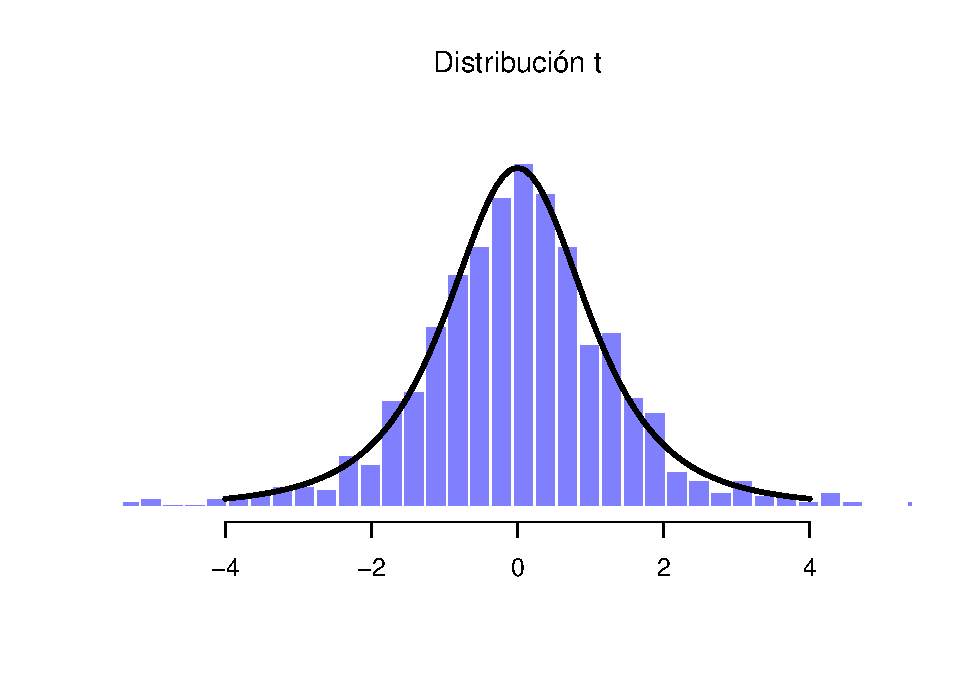
\includegraphics{FdI2_files/figure-latex/distt-1.pdf}
\caption{\label{fig:distt}Distribución t. Es el resultado de dividir una
distribución normal (en este caso la Muestra D) entre una variable
chi-cuadrada escalada}
\end{figure}

Del mismo modo, podemos obtener una distribución \(F\) al dividir dos
distribuciones chi-cuadrada ``escaladas''. Supongamos, por ejemplo, que
deseamos generar datos que sigan una distribución \(F\) con 3 y 20
grados de libertad (es decir, con 3 y 20 variables respectivamente). La
división de los valores de ambas distribuciones nos da como resultado
una nueva variable \texttt{F.3.20} y su distribución es la que se
muestra en la Figura \ref{fig:distf}.

\begin{figure}
\centering
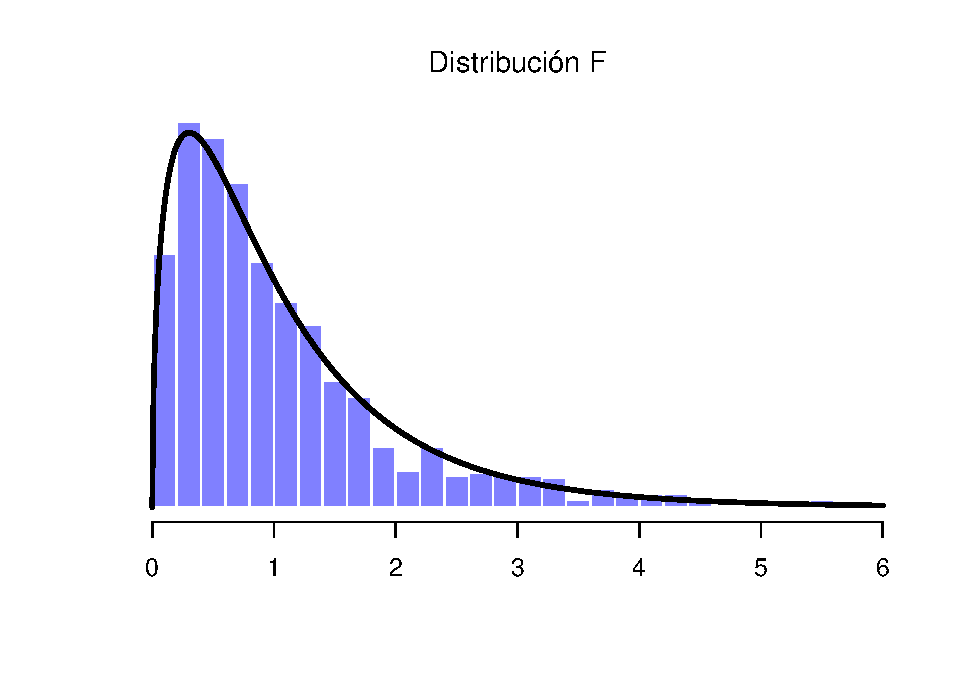
\includegraphics{FdI2_files/figure-latex/distf-1.pdf}
\caption{\label{fig:distf}Distribución F. En este ejemplo hipotético, se
compara la distribución chi-cuadrada de 3 grados de libertad previa con
otra distribución chi-cuadrada con 20 grados de libertad (es decir, que
incluye 20 muestras o variables)}
\end{figure}

Hemos visto tres nuevas distribuciones: \(\chi^2\), \(t\) y \(F\). Todas
son distribuciones continuas, y todas están estrechamente relacionadas
con la distribución normal. Hemos hablado un poco poco sobre la
naturaleza de esta relación. Sin embargo, la clave no es que tengas una
comprensión profunda y detallada de todas estas diferentes
distribuciones, ni que recuerdes las relaciones precisas que existen
entre ellas. Lo más importante es entender la idea básica de que estas
distribuciones están profundamente relacionadas entre sí y a su vez con
la distribución normal. Más adelante en el curso nos vamos a encontrar
con datos que se distribuyen normalmente, o que al menos suponemos que
se distribuyen normalmente. Por lo tanto, si suponemos que nuestros
datos se distribuyen normalmente, debemos saber reconocer las
distribuciones \(\chi^2\), \(t\) y \(F\)..

\section{Resumen}\label{resumen}

En este capítulo hemos hablado de probabilidad. Hemos hablado de lo que
significa la probabilidad y por qué los estadísticos no están muy de
acuerdo en lo que significa. Hablamos sobre las reglas que las
probabilidades tienen que obedecer. Hemos introducido la idea de una
distribución de probabilidad y conocido algunas de las distribuciones de
probabilidad más importantes con las que nos podemos encontrar. Los
temas han sido los siguientes:

\begin{itemize}
\tightlist
\item
  Teoría de probabilidad vs estadística (Sección \ref{probstats})
\item
  Visión frecuenciantista vs visión bayesiana de probabilidad (Sección
  \ref{probmeaning})
\item
  Conceptos básicos de la teoría de probabilidad (Sección
  \ref{basicprobability})
\item
  Distribución binomial (Sección \ref{binomial}), distribución normal
  (sección \ref{normal}), y otras distribuciones (Sección
  \ref{otherdists})
\end{itemize}

Esto es una simple introducción dentro de un gran tema. La teoría de la
probabilidad es una rama de las matemáticas, completamente separada de
su aplicación a la estadística y al análisis de datos. Como tales, hay
miles de libros escritos sobre el tema y las universidades generalmente
ofrecen clases dedicadas por completo a la teoría de la probabilidad. En
este capítulo se han descrito cinco distribuciones de probabilidad
estándar, pero existen \emph{muchas} más que esas. Afortunadamente,
estas distribuciones bastarán por el momento.

Los conceptos básicos que hemos adquirido en este capítulo servirán como
fundamento para los siguientes dos. Existen muchas reglas sobre lo que
se nos ``permite'' decir cuando hacemos inferencia estadística, y muchas
de ellas pueden parecer arbitrarias. Sin embargo, veremos que comienzan
a tener sentido si tenemos en cuenta estos conceptos básicos que hemos
aprendido.

\bibliography{book.bib,packages.bib}


\end{document}
